\usetikzlibrary{arrows.meta,positioning}

\begin{frame}{fast writes}
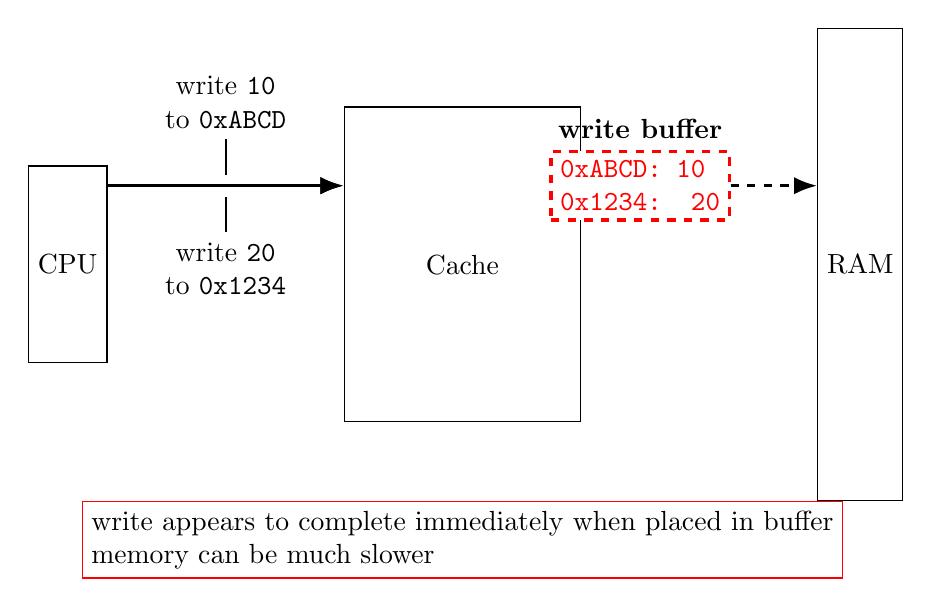
\begin{tikzpicture}
    \tikzset{every pin edge/.style={-,thick}}
\node[draw,minimum width=1cm,minimum height=2.5cm] (cpu) {CPU};
\node[draw,minimum width=3cm,minimum height=4cm,right=3cm of cpu] (cache) {Cache};
\node[draw,minimum width=1cm,minimum height=6cm,right=3cm of cache] (mem) {RAM};
\draw[very thick,-Latex] ([yshift=1cm]cpu.east) -- ([yshift=1cm]cache.west)
    node[-,midway,pin={[align=center,-]north:write {\tt 10}\\to {\tt 0xABCD}}] (cacheWrite) {};
\draw[very thick,-Latex] ([yshift=1cm]cpu.east) -- ([yshift=1cm]cache.west)
    node[-,midway,pin={[align=center,-]south:write {\tt 20}\\to {\tt 0x1234}}] (cacheWrite2) {};
\draw[very thick,dashed,-Latex] ([yshift=1cm]cache.east) coordinate (cacheOut) --
    ([yshift=1cm]mem.west) coordinate (memIn)
    node[align=left,font=\tt,red,very thick,near start,label={[font=\bfseries]write buffer},draw,fill=white] { 0xABCD: 10 \\ 0x1234: 20 };

    \node[draw=red,fill=white,below=1cm of cache,align=left] { write appears to complete immediately when placed in buffer \\ memory can be much slower};
\end{tikzpicture}
\end{frame}
